\documentclass[../main.tex]{subfiles}
\begin{document}

\section{Introduzione}

In questo capitolo verranno descritti gli esperimenti effettuati utilizzando modelli e tecniche proposti nel capitolo precedente per valutare le prestazioni sul dataset KvasirVQA, con un approfondimento sulla parte tecnica e sulle implementazioni adottate.

\section{Setup degli esperimenti}

\subsection{Configurazione hardware}L'addestramento è stato eseguito su un computer con una configurazione non professionale né ottimale per il compito:  

\begin{itemize}
    \item \textbf{GPU}: NVIDIA RTX3060Ti con 8GB di memoria, sfruttando il supporto per il calcolo parallelo che ha permesso di ridurre i tempi di calcolo sfruttando i CUDA cores.
    \item \textbf{CPU}: Intel i7 12700KF.
    \item \textbf{RAM}: 32GB di RAM DDR4.
\end{itemize}

\subsection{Configurazione software}

Per quanto riguarda la configurazione software, sono state utilizzate in primis le librerie solitamente più gettonate in ambito \textit{Machine Learning} e \textit{AI}, ovvero:

\begin{itemize}
    \item \textit{Scikit-learn} per la possibilità di richiamare le API funzionali per il calcolo delle metriche, creazione di \textit{classification report} e divisione dei dati in split per gli addestramenti.
    \item \textit{Seaborn e Matplotlib} per la visualizzazione di dati e grafici, in particolare dei report creati dalle librerie di \textit{Scikit-learn}.
    \item \textit{PyTorch} per la scrittura di modelli personalizzati, manipolazione dei tensori, implementazione di metodi per inferenza e creazione dei loop di addestramento.
    \item \textit{HuggingFace} per la possibilità di avvalersi dei modelli caricati sulla piattaforma, ma anche delle API per il recupero dei dataset e utilizzo dei modelli transformers e i loro tokenizzatori.
    \item \textit{NumPy e Pandas} per la manipolazione delle strutture dati, in particolare dei \textit{DataFrame} Pandas.
    \item \textit{NLTK e pycocoevalcap} per operazioni sul testo come tokenizzazione e calcolo del CIDEr score.
\end{itemize} 

Infine, per sfruttare al meglio la configurazione hardware e in particolare la GPU per l'accelerazione hardware, è stato configurato un ambiente software con CUDA versione 12.6.
Per un fattore di riproducibilità, ove possibile, è stato impostato manualmente il valore di \textit{seed} uguale a 42.

\section{Preprocessing dei dati}

In base alla dimensionalità degli input delle varie architetture, sono state necessarie delle operazioni di preprocessing, più o meno simili tra loro.
Inoltre, grazie alle operazioni di data augmentation descritte, è stato possibile effettuare addestramenti e poi esperimenti stratificando gli split di addestramento, test e validazione in base alle domande. 
In particolare, il 70\% dei dati del KvasirVQA è stato utilizzato per l'addestramento, il restante 30\% è stato ripartito in parti uguali per la validazione dei modelli e per i test.

\subsection{ViLT}

Come accennato nel capitolo precedente, l'operazione di preprocessing in questo caso viene svolta avvalendosi del processor di ViLT, utilizzabile grazie alle API di \textit{HuggingFace}, che va quindi a effettuare una normalizzazione dell'immagine e ad aggiungere una maschera per il padding in base alle dimensioni del resto delle immagini nella batch.

\subsection{Modelli custom}

Per le architetture custom che sono state descritte nello scorso capitolo, si è scelto di adottare un approccio di preprocessing comune, ovvero una pipeline con le seguenti trasformazioni provenienti dalla libreria \textit{v2} di \textit{torchvision.transforms}:

\begin{itemize}
    \item \textbf{v2.Resize}: ridimensionamento delle immagini a 224x224, per l'adattamento alle dimensioni di input delle reti.
    \item \textbf{v2.toDtype} e \textbf{v2.Normalize}: per la trasformazione dei valori dei pixel.
\end{itemize}

\subsection{Altre architetture}

Per il preprocessing dei dati da fornire in input agli altri modelli, sono stati utilizzati i processor associati e disponibili su HuggingFace, che coprono autonomamente la parte relativa al resize dell'immagine, aggiunta eventuale di maschere per il padding, normalizzazione del valore dei pixel ed eliminazione di bordi indesiderati.

\section{Metriche di valutazione}

Per la valutazione della bontà dei modelli scelti, sono stati utilizzati due insiemi di metriche, distinguendo per i task di generazione del testo assistito da prompting e classificazione.

\subsection{Task di classificazione}

Per la valutazione dei task di classificazione è stata scelta la metrica dell'\textit{F1 Score}, una metrica di valutazione utilizzata per misurare l'equilibrio tra \textit{Precision} e \textit{Recall} in un modello di classificazione. 
È particolarmente utile quando, come nel nostro caso, le classi sono sbilanciate, poiché fornisce una media armonica di Precision e Recall.

La formula dell'F1 Score è la seguente:

\[
F1 = 2 \cdot \frac{\text{Precision} \cdot \text{Recall}}{\text{Precision} + \text{Recall}}
\]

Dove:
\begin{itemize}
    \item \textbf{Precision:} La frazione di esempi predetti positivi che sono effettivamente positivi.
    \item \textbf{Recall:} La frazione di esempi positivi correttamente identificati come tali.
\end{itemize}

L'F1 Score assume valori compresi tra 0 e 1, per cui valori più vicini a 1 indicano un buon equilibrio tra Precision e Recall, mentre valori più bassi suggeriscono che il modello è meno efficace nel bilanciare i falsi positivi e i falsi negativi.

Nel contesto della classificazione multilabel, l'F1 Score può essere calcolato per ogni classe e successivamente aggregato come media macro o pesata in base alla frequenza delle classi. 
I risultati mostrati saranno il risultato dell'F1 Score con media macro.

\subsection{Task generativi}

Per i task di generazione del testo, sono state scelte in particolare le stesse metriche presenti nel paper originale del KvasirVQA, in modo da fornire un confronto coerente con le prestazioni dichiarate dagli autori che si sono avvalsi di un modello \textit{Florence-2} riaddestrato sui propri dati.

\subsubsection{BLEU} 

BLEU \cite{10.3115/1073083.1073135} è una metrica automatica utilizzata per valutare la qualità dei testi generati da modelli di linguaggio o traduzione rispetto a un riferimento umano. Misura la somiglianza tra il testo generato e uno o più testi di riferimento, calcolando il numero di n-grammi condivisi.
Sfruttando gli n-grammi, ovvero sequenze di \textit{n} elementi uguali da un testo, è indipendente dalla lingua scelta e favorisce la corrispondenza tra quegli n-grammi di lunghezza maggiore, come i bi e trigrammi.
Inoltre, è progettato in modo da essere uno score normalizzato da 0 a 1 o da 0 a 100 in caso di scala percentuale, per una maggiore interpretabilità del punteggio.
Non avendo tuttavia comprensione della semantica, non gestisce bene risposte semanticamente simili o che rappresentano una parafrasi della risposta reale.

\paragraph{Formula:}
\[
BLEU = BP \cdot \exp \left( \sum_{n=1}^{N} w_n \log P_n \right)
\]
Dove:
\begin{itemize}
    \item \(P_n\): precisione degli n-grammi condivisi.
    \item \(w_n\): peso associato a ogni n-gramma (spesso uguale per tutti).
    \item \(BP\): brevity penalty, penalizza risposte troppo brevi rispetto al riferimento.
\end{itemize}

\subsubsection{METEOR}

METEOR \cite{article} è una metrica progettata per valutare la qualità delle traduzioni automatiche confrontando il testo generato con una traduzione di riferimento. 

Grazie alla sua capacità di riconoscere variazioni lessicali e semantiche, METEOR è ampiamente utilizzata in campi come la traduzione automatica e il riepilogo testuale. Rispetto ad altre metriche, METEOR è particolarmente sensibile alle differenze linguistiche e alle variazioni di formulazione, risultando più rappresentativa della qualità percepita dall'utente finale e dimostra una maggiore potenzialità nel riconoscere variazioni lessicali e semantiche.

\paragraph{Formula}
La metrica combina precisione (\(P\)) e richiamo (\(R\)) utilizzando una media armonica pesata, calcolata come:
\[
F_{\text{mean}} = \frac{10 \cdot P \cdot R}{9 \cdot P + R}.
\]
Successivamente, viene applicata una penalità per penalizzare disordini strutturali nella traduzione:
\[
\text{METEOR} = F_{\text{mean}} \cdot (1 - P_\text{penalty}).
\]

\subsubsection{ROUGE}

ROUGE \cite{lin-2004-rouge} è una metrica comunemente utilizzata per valutare la qualità dei riassunti automatici e di altri compiti di generazione testuale. 
Si basa sul confronto tra le unità linguistiche (ad esempio, parole o frasi) generate automaticamente e quelle presenti in un testo di riferimento, privilegiando il richiamo (\textit{recall}) come indicatore principale.

La famiglia di metriche ROUGE comprende diverse varianti, quelle che sono state utilizzate all'interno della tesi, in particolare, sono:

\begin{itemize}
    \item \textbf{ROUGE-1}, che calcola il richiamo di unigrams (parole singole) condivisi tra il testo generato e il riferimento. È particolarmente utile per valutare la copertura lessicale di base.
    \item \textbf{ROUGE-2}, che misura il richiamo di bigrammi (sequenze di due parole consecutive), offrendo un'analisi più dettagliata della fluidità e della continuità testuale.
    \item \textbf{ROUGE-L}, che utilizza la lunghezza della sottosequenza comune più lunga (\textit{Longest Common Subsequence}, LCS) per valutare la similarità strutturale tra i testi. Questa variante tiene conto della coerenza globale.
    \item \textbf{ROUGE-L-SUM}, una variante di ROUGE-L che è specificamente progettata per valutare riassunti generati automaticamente, considerando simultaneamente l'allineamento strutturale e la copertura delle informazioni chiave.
\end{itemize}

Ad esempio, ROUGE-1 e ROUGE-2 calcolano il richiamo rispettivamente di unigrams e bigrammi:
\[
\text{ROUGE-N} = \frac{\text{n-grammi comuni}}{\text{n-grammi nel riferimento}}.
\]

ROUGE-L, invece, si concentra sulla lunghezza della sottosequenza comune più lunga, considerando l'ordine delle parole e non solo la loro presenza. Questa metrica è particolarmente utile nei casi in cui si voglia valutare la capacità del modello di mantenere una struttura coerente con il riferimento.

ROUGE-L-SUM rappresenta un'estensione specifica per i riassunti e bilancia l'importanza delle informazioni chiave e della struttura.

Nel contesto della tesi, queste varianti sono state utilizzate per analizzare diverse sfaccettature delle risposte generate dai modelli. ROUGE-1 e ROUGE-2 valutano la corrispondenza lessicale e la fluidità locale, mentre ROUGE-L e ROUGE-L-SUM analizzano la coerenza strutturale e l'adeguatezza delle informazioni. I dati riportati nelle tabelle per la metrica ROUGE riguarderanno in particolare ROUGE-1.

\subsubsection{CIDEr}

CIDEr \cite{vedantam2015ciderconsensusbasedimagedescription} è una metrica progettata per valutare la qualità delle descrizioni generate automaticamente per le immagini. Si basa sul confronto tra una descrizione generata e un insieme di descrizioni di riferimento, ponendo un'enfasi particolare sul consenso tra le descrizioni umane.

La metrica calcola un punteggio basato sulla similarità tra n-grammi della descrizione generata e delle descrizioni di riferimento, ponderando ciascun n-gramma in base alla sua frequenza nei dati di riferimento. Nello specifico, CIDEr assegna maggior peso agli n-grammi che appaiono frequentemente nelle descrizioni di riferimento, ma che non sono troppo comuni nei testi generali, utilizzando il \textit{Term Frequency-Inverse Document Frequency} (TF-IDF) come schema di ponderazione. TF-IDF misura l'importanza di un termine nel contesto di un documento specifico, penalizzando i termini troppo frequenti nel corpus (che portano poca informazione discriminante) e premiando quelli rari, ma significativi.

Il calcolo del punteggio CIDEr può essere riassunto nei seguenti passaggi:
\begin{itemize}
    \item Ogni descrizione viene rappresentata come un insieme di n-grammi, con $n$ che varia tra 1 e 4.
    \item Per ciascun n-gramma, viene calcolata una ponderazione basata sul TF-IDF, che misura la sua rilevanza nel contesto delle descrizioni di riferimento.
    \item Si calcola la similarità tra le descrizioni generate e quelle di riferimento utilizzando la somma ponderata delle similarità degli n-grammi condivisi.
    \item Infine, il punteggio viene mediato su tutte le descrizioni di riferimento per ottenere una misura complessiva di consenso.
\end{itemize}

CIDEr è particolarmente adatto per task di descrizione delle immagini, poiché tiene conto sia della specificità del linguaggio utilizzato sia della coerenza semantica rispetto ai riferimenti umani. 

\paragraph{Formula}

La formula del CIDEr per un singolo n-gramma è data da:
\[
\text{CIDEr}(c, S) = \frac{1}{|S|} \sum_{s \in S} \frac{\text{TF-IDF}(c) \cdot \text{TF-IDF}(s)}{\|\text{TF-IDF}(c)\| \|\text{TF-IDF}(s)\|},
\]
dove $c$ rappresenta la descrizione generata, $S$ l'insieme delle descrizioni di riferimento e $\text{TF-IDF}$ è il peso assegnato a ciascun n-gramma.

\cite{vedantam2015ciderconsensusbasedimagedescription}

\section{Risultati}

A seguire, mostreremo i risultati sperimentali ottenuti testando le varie configurazioni. 
Distingueremo le configurazioni che hanno previsto un addestramento, come nel caso di ViLT e dell'architettura personalizzata, dalle configurazioni che hanno sfruttato tecniche di prompting: verranno chiaramente fatte valutazioni distinte in base alle metriche utilizzate e alle differenze riscontrate tra gli addestramenti e la fase di inferenza, dal momento che queste differenze sono ritenute un riflesso della distribuzione sbilanciata dei dati all'interno del dataset.

\subsection{ViLT - Multiclasse}

\begin{figure}[H]
    \centering
    \includegraphics[width=1\linewidth]{static//vilt-multiclass/run.png}
    \caption{Grafico dell'andamento dell'addestramento multiclasse per il modello ViLT based}
    \label{fig:enter-label}
\end{figure}

\textbf{F1-Score}: 0.5955

\subsection{ViLT - Multilabel}

\begin{figure}[H]
    \centering
    \includegraphics[width=1\linewidth]{static//vilt-multilabel/run.png}
    \caption{Grafico dell'andamento dell'addestramento multilabel per il modello ViLT based}
    \label{fig:enter-label}
\end{figure}

\textbf{F1-Score}: 0.5369

\subsection{Custom - Multiclasse}

\begin{figure}[H]
    \centering
    \includegraphics[width=1\linewidth]{static//custom-multiclass/run.png}
    \caption{Grafico dell'andamento dell'addestramento dell'architettura custom per task di classificazione multiclasse}
    \label{fig:enter-label}
\end{figure}

\textbf{F1-Score}: 0.0369

\subsection{Custom - Multilabel}

\begin{figure}[H]
    \centering
    \includegraphics[width=1\linewidth]{static//custom-multilabel/run.png}
    \caption{Grafico dell'andamento dell'addestramento dell'architettura custom per task di classificazione multilabel}
    \label{fig:enter-label}
\end{figure}

\textbf{F1-Score}: 0.3944. 

\subsection{Classificazione}

\begin{table}[H]
    \centering
    \begin{tabular}{|l|c|c|c|c|}
    \hline
    \textbf{Modello} &
    \textbf{Task} &
    \textbf{F1-Score} \\ \hline
    Custom & Multiclasse & 0.0369 \\ \hline
    Custom & Multilabel & 0.3944 \\ \hline
    ViLT & Multiclasse & 0.5369 \\ \hline
    ViLT & Multilabel & 0.5955 \\ \hline
    \end{tabular}
    \caption{Tabella riassuntiva delle prestazioni dei vari modelli usati per task di classificazione}
    \label{tab:recap-classify}
\end{table}

La Tabella \ref{tab:recap-classify} presenta un riepilogo delle prestazioni ottenute dai modelli testati nei task di classificazione multiclasse e multilabel, valutati tramite l'F1-Score. I risultati mettono in evidenza significative differenze tra le due configurazioni di task e tra le architetture considerate.

Il modello \textit{Custom}, progettato per essere specifico al dataset KvasirVQA, ha mostrato un F1-Score particolarmente basso nel task di classificazione multiclasse (0.0369), evidenziando difficoltà nel catturare le relazioni tra le immagini e le etichette di risposta in un contesto altamente discreto come quello multiclasse. Questo risultato può essere attribuito alla natura complessa del dataset, caratterizzata da una distribuzione di classi estremamente sbilanciata e da un numero elevato di risposte possibili, che ricordiamo essere 469. 
Inoltre, si osserva una discrepanza notevole tra l'accuracy durante la fase di addestramento e quella nella fase di test, suggerendo che il modello fatichi a generalizzare in questa configurazione.

Nel task di classificazione multilabel, il modello \textit{Custom} ha ottenuto un F1-Score pari a 0.3944, dimostrando un netto miglioramento rispetto alla configurazione multiclasse. Questo punteggio riflette il vantaggio dell'approccio multilabel nel trattare risposte che coinvolgono combinazioni multiple di classi, più adatte alla struttura del dataset in analisi. Il miglioramento ottenuto conferma che il task multilabel consente di rappresentare in modo più accurato le complessità intrinseche del problema, riducendo al contempo le difficoltà legate alla rigidità delle classificazioni multiclasse.

Il modello \textit{ViLT} ha ottenuto risultati nettamente migliori rispetto al \textit{Custom}, sia nel task multiclasse (F1-Score di 0.5369) sia in quello multilabel (F1-Score di 0.5955). In particolare, il passaggio al task multilabel ha prodotto un miglioramento significativo, dimostrando che questa configurazione consente al modello di esprimere in modo migliore il suo potenziale. 
Tuttavia, anche nel caso di ViLT, si osserva una certa discrepanza tra l'accuracy in fase di addestramento e quella nella fase di test. Questo fenomeno, condiviso con il modello \textit{Custom}, è attribuibile alle caratteristiche del dataset.

Questi risultati sottolineano come la scelta del task e dell'architettura influenzi in modo significativo le performance. L'approccio multilabel si è dimostrato più adatto per il dataset KvasirVQA, grazie alla maggiore flessibilità nel rappresentare risposte complesse e composizioni multiclasse. Sebbene il modello \textit{Custom} abbia mostrato un miglioramento apprezzabile nel task multilabel, il divario rispetto a \textit{ViLT} evidenzia la necessità di ulteriori ottimizzazioni, sia a livello architetturale che di pre-elaborazione dei dati. 
Inoltre, il confronto mette in luce il valore aggiunto offerto dai modelli pre-addestrati su dataset di grandi dimensioni, i quali sono in grado di generalizzare meglio a problemi specifici anche in presenza di dataset complessi e sbilanciati come il KvasirVQA.

\subsection{Prompting}

\begin{table}[H]
    \centering
    \begin{tabular}{|l|c|c|c|c|c|}
    \hline
    \textbf{Modello} &
    \textbf{Prompting} &
    \textbf{BLEU} &
    \textbf{ROUGE} &
    \textbf{CIDEr} &
    \textbf{METEOR} \\ \hline
    LLaVA & template-1 & 0.0 & 0.3692 & 0.0 & 0.1961 \\ \hline
    LLaVA & template-2 & 0.0 & 0.3797 & 0.0 & 0.2041 \\ \hline
    LLaVA & cot-1 & 0.0 & 0.1364 & 0.0 & 0.0617 \\ \hline
    LLaVA & cot-2 & 0.0 & 0.3893 & 0.0 & 0.2034 \\ \hline
    GIT & template-1 & 0.0 & 0.059 & 0.0 & 0.0288 \\ \hline
    GIT & template-2 & 0.0 & 0.0033 & 0.0 & 0.001 \\ \hline
    GIT & cot-1 & 0.0 & 0.0003 & 0.0 & 0.0001 \\ \hline
    GIT & cot-2 & 0.0 & 0.0046 & 0.0 & 0.0002 \\ \hline
    BLIP & template-1 & 0.0 & 0.1266 & 0.0 & 0.1266 \\ \hline
    BLIP & template-2 & 0.0 & 0.158 & 0.0 & 0.0798 \\ \hline
    BLIP & cot-1 & 0.0 & 0.1009 & 0.0 & 0.0441 \\ \hline
    BLIP & cot-2 & 0.0 & 0.1192 & 0.0 & 0.0606 \\ \hline
    \end{tabular}
    \caption{Tabella riassuntiva dei risultati dei modelli con tecniche di prompting}
    \label{tab:prompting}
\end{table}

\subsubsection{Analisi delle performance per modello}

Il \textbf{modello LLaVA} si distingue come il più performante, raggiungendo i migliori punteggi per ROUGE e METEOR in quasi tutte le configurazioni. In particolare, con il prompting basato su template-2, LLaVA ottiene un ROUGE pari a 0.3797 e un METEOR di 0.2041, dimostrando un'elevata coerenza e rilevanza semantica nelle risposte generate. Anche utilizzando CoT-2, il modello mantiene prestazioni competitive, con un ROUGE pari a 0.3893 e un METEOR di 0.2034, mostrando una certa versatilità nell'adattarsi a diversi tipi di prompting.

Il \textbf{modello BLIP} presenta risultati più modesti rispetto a LLaVA, ma comunque significativi. Con il prompting template-2, raggiunge un ROUGE di 0.158 e un METEOR di 0.0798, dimostrando una discreta capacità di generare risposte contestualmente rilevanti. Tuttavia, i risultati con CoT sono inferiori, con un massimo di 0.1192 per ROUGE e 0.0606 per METEOR, suggerendo che il modello non beneficia pienamente di questa tecnica.

Infine, il \textbf{modello GIT} registra i risultati più bassi in tutte le metriche. Anche nella configurazione migliore (template-1), ottiene un ROUGE di appena 0.059 e un METEOR di 0.0288. I punteggi estremamente bassi con CoT (ROUGE massimo di 0.0046 e METEOR massimo di 0.0002) indicano difficoltà significative nel comprendere e generare risposte coerenti, indipendentemente dal prompting utilizzato.

\subsubsection{Confronto tra template e Chain-of-Thought}

Le tecniche di prompting basate su template si dimostrano generalmente più efficaci rispetto a quelle basate su Chain-of-Thought. Per LLaVA, ad esempio, template-2 ottiene punteggi leggermente superiori rispetto a CoT-2 in METEOR (0.2041 contro 0.2034) e ROUGE (0.3797 contro 0.3893), pur mantenendo un margine molto ridotto. BLIP evidenzia una differenza più marcata, con template-2 che supera CoT sia in ROUGE che in METEOR, indicando che il modello risponde meglio a prompt strutturati piuttosto che a strategie di ragionamento esplicito. GIT, al contrario, non beneficia significativamente di nessuna delle tecniche, confermando le sue limitazioni.

\subsubsection{Osservazioni generali}

L'assenza di punteggi positivi per BLEU e CIDEr solleva interrogativi sulla capacità dei modelli di generare risposte strettamente correlate ai riferimenti testuali. Questo fenomeno potrebbe essere attribuito a un disallineamento tra i prompt utilizzati e la struttura delle risposte attese, o a limiti intrinseci nei modelli testati. 

Inoltre, i punteggi relativamente bassi per ROUGE e METEOR, specialmente per BLIP e GIT, indicano che i modelli non riescono a catturare completamente la complessità semantica richiesta dal task. Tuttavia, LLaVA si distingue come il modello più promettente, suggerendo che ulteriori ottimizzazioni, come un miglioramento del design dei template o un fine-tuning specifico, potrebbero ulteriormente migliorare le sue prestazioni.

In conclusione, LLaVA si dimostra il modello più efficace per i task generativi testati, mentre BLIP e, soprattutto, GIT mostrano prestazioni limitate. Le tecniche di templating emergono come la scelta più solida rispetto a Chain-of-Thought, evidenziando la necessità di un prompting ben strutturato per massimizzare le capacità dei modelli in contesti complessi. Tuttavia, l'assenza di risultati significativi per BLEU e CIDEr sottolinea l'importanza di ulteriori analisi e ottimizzazioni.

\subsection{Criticità}

Durante l'utilizzo delle tecniche di prompting, sono emerse diverse criticità che hanno evidenziato le sfide di questo approccio. 
Una delle principali difficoltà è stata la formulazione dei prompt, sia per quanto riguarda il \textit{templating} che il \textit{Chain-of-Thought} (CoT). 
Per il \textit{templating}, la sfida era creare una struttura standardizzata e sufficientemente chiara per guidare il modello nella generazione di risposte pertinenti. Piccole variazioni nella formulazione, come l'ordine delle parole o la presentazione delle opzioni, hanno avuto un impatto significativo sulle prestazioni, mostrando una forte dipendenza del modello dalla struttura del prompt. 
Nel caso del CoT, l'equilibrio tra un livello di dettaglio sufficiente per supportare il ragionamento passo-passo e la sintesi necessaria per evitare ridondanze si è dimostrato complesso da raggiungere. 
Prompt troppo dettagliati hanno portato a risposte prolisse e inefficaci, mentre prompt più sintetici spesso non fornivano abbastanza supporto per una corretta elaborazione del ragionamento. 
Un ulteriore problema significativo è stato il fenomeno delle \textit{allucinazioni}, ovvero risposte slegate dai dati di input o dalle istruzioni fornite. Questo è risultato particolarmente evidente in task con domande aperte o opzioni multiple, dove il modello, pur essendo guidato da prompt che specificavano di rispondere utilizzando solo le opzioni fornite, talvolta generava risposte che non appartenevano al vocabolario previsto. 
Infine, un aspetto non trascurabile è stato rappresentato dai costi computazionali. Sebbene il prompting eviti il processo di \textit{fine-tuning}, il tempo necessario per iterare e testare diverse versioni di prompt, combinato con l'elaborazione passo-passo richiesta dal CoT, ha portato a un utilizzo significativo di risorse. Questo sottolinea come, nonostante i vantaggi in termini di flessibilità e scalabilità, l'adozione di tecniche di prompting richieda comunque un impegno computazionale rilevante. 

Per quanto riguarda invece il fine-tuning dei modelli, sono emerse criticità altrettanto significative legate principalmente alla dipendenza da un dataset robusto e corposo.
L'addestramento dei modelli si è rivelato fortemente influenzato dalla qualità e dalla quantità dei dati disponibili, evidenziando che dataset con distribuzioni sbilanciate o categorie sottorappresentate possono limitare significativamente le capacità generative e di generalizzazione del modello. 
Questo aspetto si è mostrato particolarmente problematico nel caso di task di classificazione multiclasse, dove l'elevato numero di classi ha richiesto al modello di apprendere un'enorme varietà di combinazioni di risposte, aumentando notevolmente la complessità del processo di addestramento. 
La presenza di classi con pochissimi esempi ha portato inoltre a una maggiore probabilità di errore, richiedendo strategie di \textit{data augmentation} per migliorare l'equilibrio tra le categorie. 
Un'altra criticità significativa riguarda la rigidità dei modelli che hanno subito fine-tuning, i quali, a differenza di approcci basati sul prompting, perdono la loro capacità di adattarsi dinamicamente a nuovi task o domini senza ulteriori cicli di addestramento. 
Questa rigidità rappresenta un limite importante, soprattutto in contesti dove le domande o i dati di input possono variare in modo significativo rispetto al set di addestramento. 
Inoltre, il fine-tuning comporta costi temporali e computazionali elevati: la necessità di eseguire molteplici iterazioni di addestramento su GPU di fascia alta, combinata con la ricerca di iperparametri ottimali, ha richiesto un impegno notevole in termini di risorse. 
Anche il monitoraggio continuo di metriche come la \textit{loss} e l'\textit{accuracy} o la sperimentazione di tecniche di regolarizzazione per evitare fenomeni di \textit{overfitting} ha rappresentato una sfida, soprattutto considerando la relativa esiguità del dataset KvasirVQA rispetto ad altri più ampi come MSCOCO.
Infine, nonostante il fine-tuning abbia permesso di ottenere modelli più specializzati e in grado di raggiungere prestazioni competitive, il trade-off tra flessibilità e specializzazione rimane un punto cruciale da considerare. 
Queste criticità evidenziano come, per sfruttare appieno il potenziale del fine-tuning, sia necessaria una pianificazione dettagliata che includa dataset sufficientemente diversificati e strategie di ottimizzazione mirate, bilanciando al contempo costi e benefici nel contesto applicativo specifico.

Complessivamente, queste criticità offrono importanti spunti di riflessione per migliorare l'efficacia del prompting e ottimizzare i suoi costi, aprendo nuove strade per future ricerche in questo ambito. 

\subsection{Visualizzazione attivazioni GradCAM}

Per comprendere meglio come una rete neurale convoluzionale come la \textit{ResNet-50}, pre-addestrata su ImageNet e riaddestrata su HyperKvasir e KvasirInstrument, elabora le immagini e quali regioni visive considera rilevanti durante l'estrazione delle caratteristiche, è stato utilizzato l'algoritmo \textit{Grad-CAM}, per evidenziare le aree di maggiore attivazione che influenzano le decisioni del modello.

In questa analisi, la ResNet-50 è stata utilizzata come feature extractor globale, e le sue attivazioni sono state analizzate per due immagini rappresentative provenienti dal dataset KvasirVQA. Le immagini selezionate includono un'immagine con un polipo e una con uno strumento.

\begin{figure}[H]
    \centering
    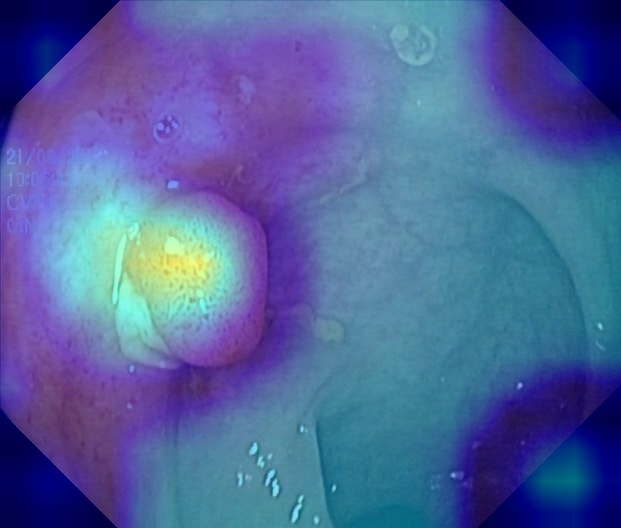
\includegraphics[width=0.5\linewidth]{static/cam_image_polyp.jpg}
    \caption{Visualizzazione delle attivazioni in immagine con polipo della ResNet-50 tramite Grad-CAM.}
    \label{fig:gradcam-polyp}
\end{figure}

\begin{figure}[H]
    \centering
    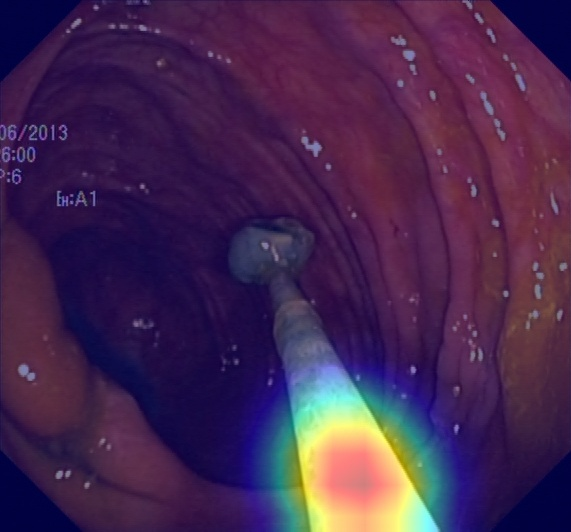
\includegraphics[width=0.5\linewidth]{static/cam_image_instrument.jpg}
    \caption{Visualizzazione delle attivazioni in immagine con strumento della ResNet-50 tramite Grad-CAM.}
    \label{fig:gradcam-instrument}
\end{figure}

Nella Figura \ref{fig:gradcam-polyp}, l'heatmap generata da Grad-CAM evidenzia lievemente la regione contenente l'anomalia, indicando che il modello considera quest'area come più rilevante per l'estrazione delle caratteristiche.

Nella Figura \ref{fig:gradcam-instrument}, l'heatmap mostra una distribuzione più concentrata in una regione dell'immagine contenente sì lo strumento, ma che mantiene un certo grado di imprecisione.

L'utilizzo di Grad-CAM ha permesso di ottenere una maggiore trasparenza nel processo decisionale della ResNet-50, evidenziando le regioni visive più significative. 

\end{document}